\dcs
%
 % In many markets, organisations are competing to propose customised products, characterised by hundreds of inter-related \textit{configuration options}. 
 % As the repertoire of inter-related options can be disconcerting for many customers, \textit{Web configurators} are developed to assist them during decision making.
% As an example, Figure~\ref{fig:configurationDummy} shows a snapshot of a typical car configurator (the circled letters and legend can be ignored for now). 
 A Web configurator provides an interactive graphical user interface that guides the users through the configuration process, verifies constraints between options, propagates user decisions, and handles conflictual decisions~\cite{ebrahimCSMR2014}. %ebrahim2013}. %rogoll2004,streichsbier2009,Trentin2012}.
% Configurators are used in many applications to personalize products and services. 
 Configurators are used in installation wizards, preference managers, and extensively used in product lines. 
 %  
 The database maintained by Cyledge is a striking evidence with 900+ Web configurators coming from 30+ different industry sectors~\cite{configurators}. % ~\cite{configurators}
% \footnote{\url{http://www.configurator-database.com}}

% Since 2007, Cyledge collected more than 900 Web configurators coming from 30+ different industry sectors, including automotive, apparel, sport, and art. 
% 
 A very simple excerpt of a real-world Web configurator is depicted in the Figure below. % ~\ref{fig:configurationDummy}. 
We can observe that the selection of \textsf{Diesel} has lead to the automated selection of \textsf{EDC6}. (In fact, some other equipment options have been previously selected; one can select \textsf{Diesel} with \textsf{EDC7} or \textsf{BVM} in some other configuration settings.) 
That is, a customer has not chosen \textsf{EDC6}; the configurator has imposed some constraints of different natures: technical/engineering constraints, aesthetic constraints, marketing constraints, \etc


% \begin{figure}[!hts]
% \vspace*{-3mm}
% \begin{center}
% \includegraphics[scale=0.31]{img/configuratorDummy.png}
%   \vspace*{-7mm}
% \caption{Audi web SC (\texttt{http://configurator.audi.co.uk/}, Oct. 18, 2012)} %\url{
% \vspace*{-9mm}
% \label{fig:configurationDummy}
% \end{center}
% \end{figure}

\begin{figure}[!hts]
\centering
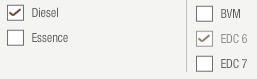
\includegraphics[scale=0.5]{figures/configuratorRenault.png}
% \vspace*{-2mm}
%\caption{{\small{Options and constraints in a configurator}}} 
% \label{fig:configurationDummy}
\vspace*{-2mm}
\end{figure}


% SCs represent a significant portion of the configurators used in modern information systems. %Their application domains range from y are used to automate the tuning of information systems to the preferences of the user. Installation wizards, preferences managers, and configurable business process models~\cite{quteprints12686,DBLP:conf/caise/GottschalkWJAR09} are examples thereof. 

% where multiple information system variants are derived from a base of reusable artefacts according to the specific characteristics of the targeted customer or market segment~\cite{Pohl2005,Schaler:2012:BIS:2363463.2363516,DBLP:conf/caise/GottschalkWJAR09,quteprints12686}. 

% A significant share of existing configurators is Web-based, irrespective of the market. 

% In this paper, we focus on web configurators supporting online sales.%, but we will argue that some of our findings generalize to other types of configurators.




% These configurators vary significantly. They each have their own characteristics, spanning visual
% aspects (GUI elements) to constraint management. 
% The web SC of Audi appearing in Figure~\ref{fig:configurationDummy} is thus only one example. It displays different options through specific widgets (radio buttons and check boxes -- \textcolor{red}{ \mycirc{A}} and \textcolor{red}{\mycirc{B}}, respectively). These options can be in different states such as activated (e.g., \configopt{Privacy glass} is flagged with \checkmark) or unavailable (e.g., \configopt{Twin-pane UV and heat-insulating glass} is greyed out). Additionally, these options are organised in different tabs (e.g., \configopt{Equipment}) and sub-tabs (e.g., \configopt{Equipment packages}) which denote a series of steps (\textcolor{red}{\mycirc{C}}) in the \emph{configuration process} (e.g., \configopt{1. Model} is followed by \configopt{2. Engine}-- \textcolor{red}{\mycirc{D}}). A SC can also implement \emph{cross-cutting\footnote{We call these constraints \emph{cross-cutting} because they are often orthogonal to the hierarchy of options, sub-options, etc. supported by the configurator.} constraints} between options (\textcolor{red}{\mycirc{E}}). These are usually hidden to the user but they determine valid combinations of options. For instance, the selection of \configopt{Privacy glass} implies the deselection of \configopt{Twin-pane UV and heat-insulating glass}, meaning that the user cannot select the latter if the former is selected. 
% Moreover, descriptive information (\textcolor{red}{\mycirc{F}}) is sometimes associated to an option (e.g., its price). % of the product.

\wprv
% As privileged channels for identifying customer needs and placing orders, configurators are key assets for companies. 
 Products, options, and the underlying constraints a configurator is in charge of are key information of an organization. 
Such information is particularly interesting from the perspective of (online) \emph{market intelligence (MI)} (also called \emph{competitive intelligence}). 
MI can be defined as the "information relevant to a company's
markets, gathered and analyzed specifically for the purpose of accurate and confident decision-making in determining
market opportunity, market penetration strategy, and market development metrics." 
Lixto, a company offering data extraction tools and services for MI, showed that it is technically feasible to acquire and exploit unstructured and semi-structured data in several case studies (\eg in the domain of computers and electronics consumer goods~\cite{baumgartner2009}). % 

Most information on pricing, product availability, product options, and product constraints is potentially available on Web sales configurators.
Specifically, competitors can use this information (1) for getting a comprehensive overview of the options and constraints in the market; (2) to be (continually) informed about strengths and weaknesses of other competitors' product lines; (3) to publicly reveal a certain superiority or marketing practice, \etc
  
 Web data extraction systems~\cite{baumgartner2009,Ferrara2014} can be specialized for acquiring configurators' information. 
 Early attempts~\cite{ebrahimCSMR2014} showed that reverse engineering Web configurators is feasible. Static analysis techniques can locate templates of options and some constraints in a Web page. % The major threat for companies developing Web configurators is that the templates followed 
  Combined with crawling techniques for deep navigation and dynamic content pages, there is the potential to comprehensively gather relevant information. 
%  Though 
  In case the static and dynamic analysis of variability can be seamlessly realized, there is a risk for companies developing Web configurators to reveal trade secrets. 
% and should provide 
 % Baumgartner \etal develop data extraction techniques and tools to improve the process of
% acquiring market information~\cite{baumgartner2009}. 
% A solid layer of knowledge is fundamental
% to optimize the decision-making activities and a large
% amount of public data could be retrieved on the Web. They to . 


% In particular, using the  Suite to access, extract, clean and deliver
% data, it is possible to gather, transform and obtain data useful
% to business purposes.

% Market intelligence comprises
% as a special case competitive intelligence. Online market
% intelligence (OMI) covers all aspects of MI that are related
% to online information sources, predominantly, to the
% Web. 





% \emph{B} 

% Analysing competitors' Websites. Web configurators coming from the same industry sector most likely present products with similar characteristics (e.g., configuration options). Using our proposed Web data extraction techniques, we can acquire market information from these competitors and compare their products (e.g., price comparison,
% option comparison). 




% Wider, the process of gathering and analyzing data about products,
% customers, competitors with the goal of helping the managers
% of a company in decisional processes is commonly called Competitive
% Intelligence, and is strictly related to data mining [58]. Zanasi
% [125] was the first to introduce the possibility of acquiring these
% data, through data mining processes, on public domain information.

% Chen et al. [22] developed a platform, that works more like
% a spider than a Web Data Extraction system, which represents a
% useful tool to support Competitive Intelligence operations. In Business
% Intelligence scenarios, we ask Web Data Extraction techniques
% to satisfy two main requirements: scalability and efficient planning
% strategies because we need to extract as much data as possible
% with the smallest amount of resources in time and space.




% Comparing prices; identifying a weakness;

% Users are forced to select some options (augmenting the price)
% Users have to follow a certain workflow 

% The Crawler can play a crucial role in exploring the configuration space and extracting dynamic data from different Web configurators (comprehensiveness) 
